
%(BEGIN_QUESTION)
% Copyright 2009, Tony R. Kuphaldt, released under the Creative Commons Attribution License (v 1.0)
% This means you may do almost anything with this work of mine, so long as you give me proper credit

Determine what type of temperature sensor is shown in this pictorial diagram, and then sketch wires showing how to correctly connect the sensor to the temperature transmitter:

$$\includegraphics[width=15.5cm]{i03999x01.eps}$$

Note what types of metal each of the connecting wires should be (e.g. copper, chromel, alumel, constantan, iron, platinum, etc.).

\vskip 20pt \vbox{\hrule \hbox{\strut \vrule{} {\bf Suggestions for Socratic discussion} \vrule} \hrule}

\begin{itemize}
\item{} A problem-solving technique useful for making proper connections in pictorial circuit diagrams is to first identify the directions of all DC currents entering and exiting component terminals, as well as the respective voltage polarity marks (+,$-$) for those terminals, based on your knowledge of each component acting either as an electrical {\it source} or an electrical {\it load}.  Discuss and compare how these arrows and polarity marks simplify the task of properly connecting wires between components. 
\item{} Identify the possible result of connecting the DC loop power supply to the wrong + and $-$ terminals on the temperature transmitter, explaining how we know this is bad for the circuit.
\item{} Students very commonly mis-interpret the symbols drawn next to the input terminals of an RTD transmitter, especially the terminals which must be made common to each other at the sensor.  One of the most popular misconceptions  is to think that those terminals shown common to each other by the symbol are already joined together {\it inside the transmitter}.  Explain why this interpretation cannot be true, based on how you know 3-wire and 4-wire RTD circuits are designed to work.
\end{itemize}

\underbar{file i03999}
%(END_QUESTION)





%(BEGIN_ANSWER)

\noindent
{\bf Partial answer:}

\vskip 10pt

The sensor is a three-wire RTD.

%(END_ANSWER)





%(BEGIN_NOTES)

$$\includegraphics[width=15.5cm]{i03999x02.eps}$$

Note: other possibilities for wiring the 4-20 mA ``loop'' circuit exist, but the direction of current needs to be the same as for this circuit.  The two white wire connections on the RTD may be safely reversed. 

%INDEX% Measurement, temperature: RTD connections

%(END_NOTES)


